\header{
    \section{Ouessant} \label{ouessant}
    %
    \insertComment{Chanson de françois Budet}{}
}

\enluminure{2}{\href{https://www.youtube.com/watch?v=WCSdKV4GOHE}{Q}}{uand les} anciens voulurent partir vers le couchant
\\Ils décrochèrent un jour un bout de continent
\\Profitant d’une nuit sans visibilité
\\Finirent par tout larguer et cap sur l’Occident.
\\Après une dérive qui dura deux-mille ans
\\Se mirent à l’ancrage aux confins de l’Iroise
\\C’est la fille de Morganne qui me l’a raconté
\\C’est ainsi que naquit son île d’Ouessant
\\C’est mon île \bissimple
\\\\Quand le vent de Gwalam et les oiseaux de mer
\\Remorquent les nuages du Pays des Abers
\\Il neige de l’écume certains matins d’hiver
\\Y’a comme des flocons sur le toit des maisons
\\Et quand le mauvais temps comme un bélier sauvage
\\Vient se briser les cornes aux dentelles des roches
\\Ses guenilles accrochées aux pointes des balises
\\La sirène de brume pousse le cri de l’Île
\\C’est mon île \bissimple
\\\\C’est mon Île de Pâques et c'est ma Santorin
\\Mon atoll au soleil, c’est mon île au trésor
\\Je l’ai vue toute nue dans un voile de crachin
\\Avec au bord des yeux, pour larmes des embrums
\\Quand la Baie de Lampaul offre ses jambes folles
\\À la caresse douce du flôt qui la remonte
\\Quand le soleil de mai la rend bien moins sauvage
\\Moi je deviens l’amant de l’Île d’Ouessant
\\C’est mon île \bissimple
\breakpage
\\\\Quand les épées des phares aux lames argentées
\\Découpent dans le soir des pans d’éternité
\\Il y a dans le silence comme une résonance
\\On apprend à se taire sur le vaisseau de pierre
\\Je veux laisser posée ma tête sur son ventre
\\Et me laisser bercer le reste de mon temps
\\C’est là que j'attendrai qu’on vienne m’embarquer
\\Pour mon dernier voyage vers l’Île d’Avalon
\\C’est mon île \bissimple
\bigskip
\bigskip
\bigskip
\begin{center}
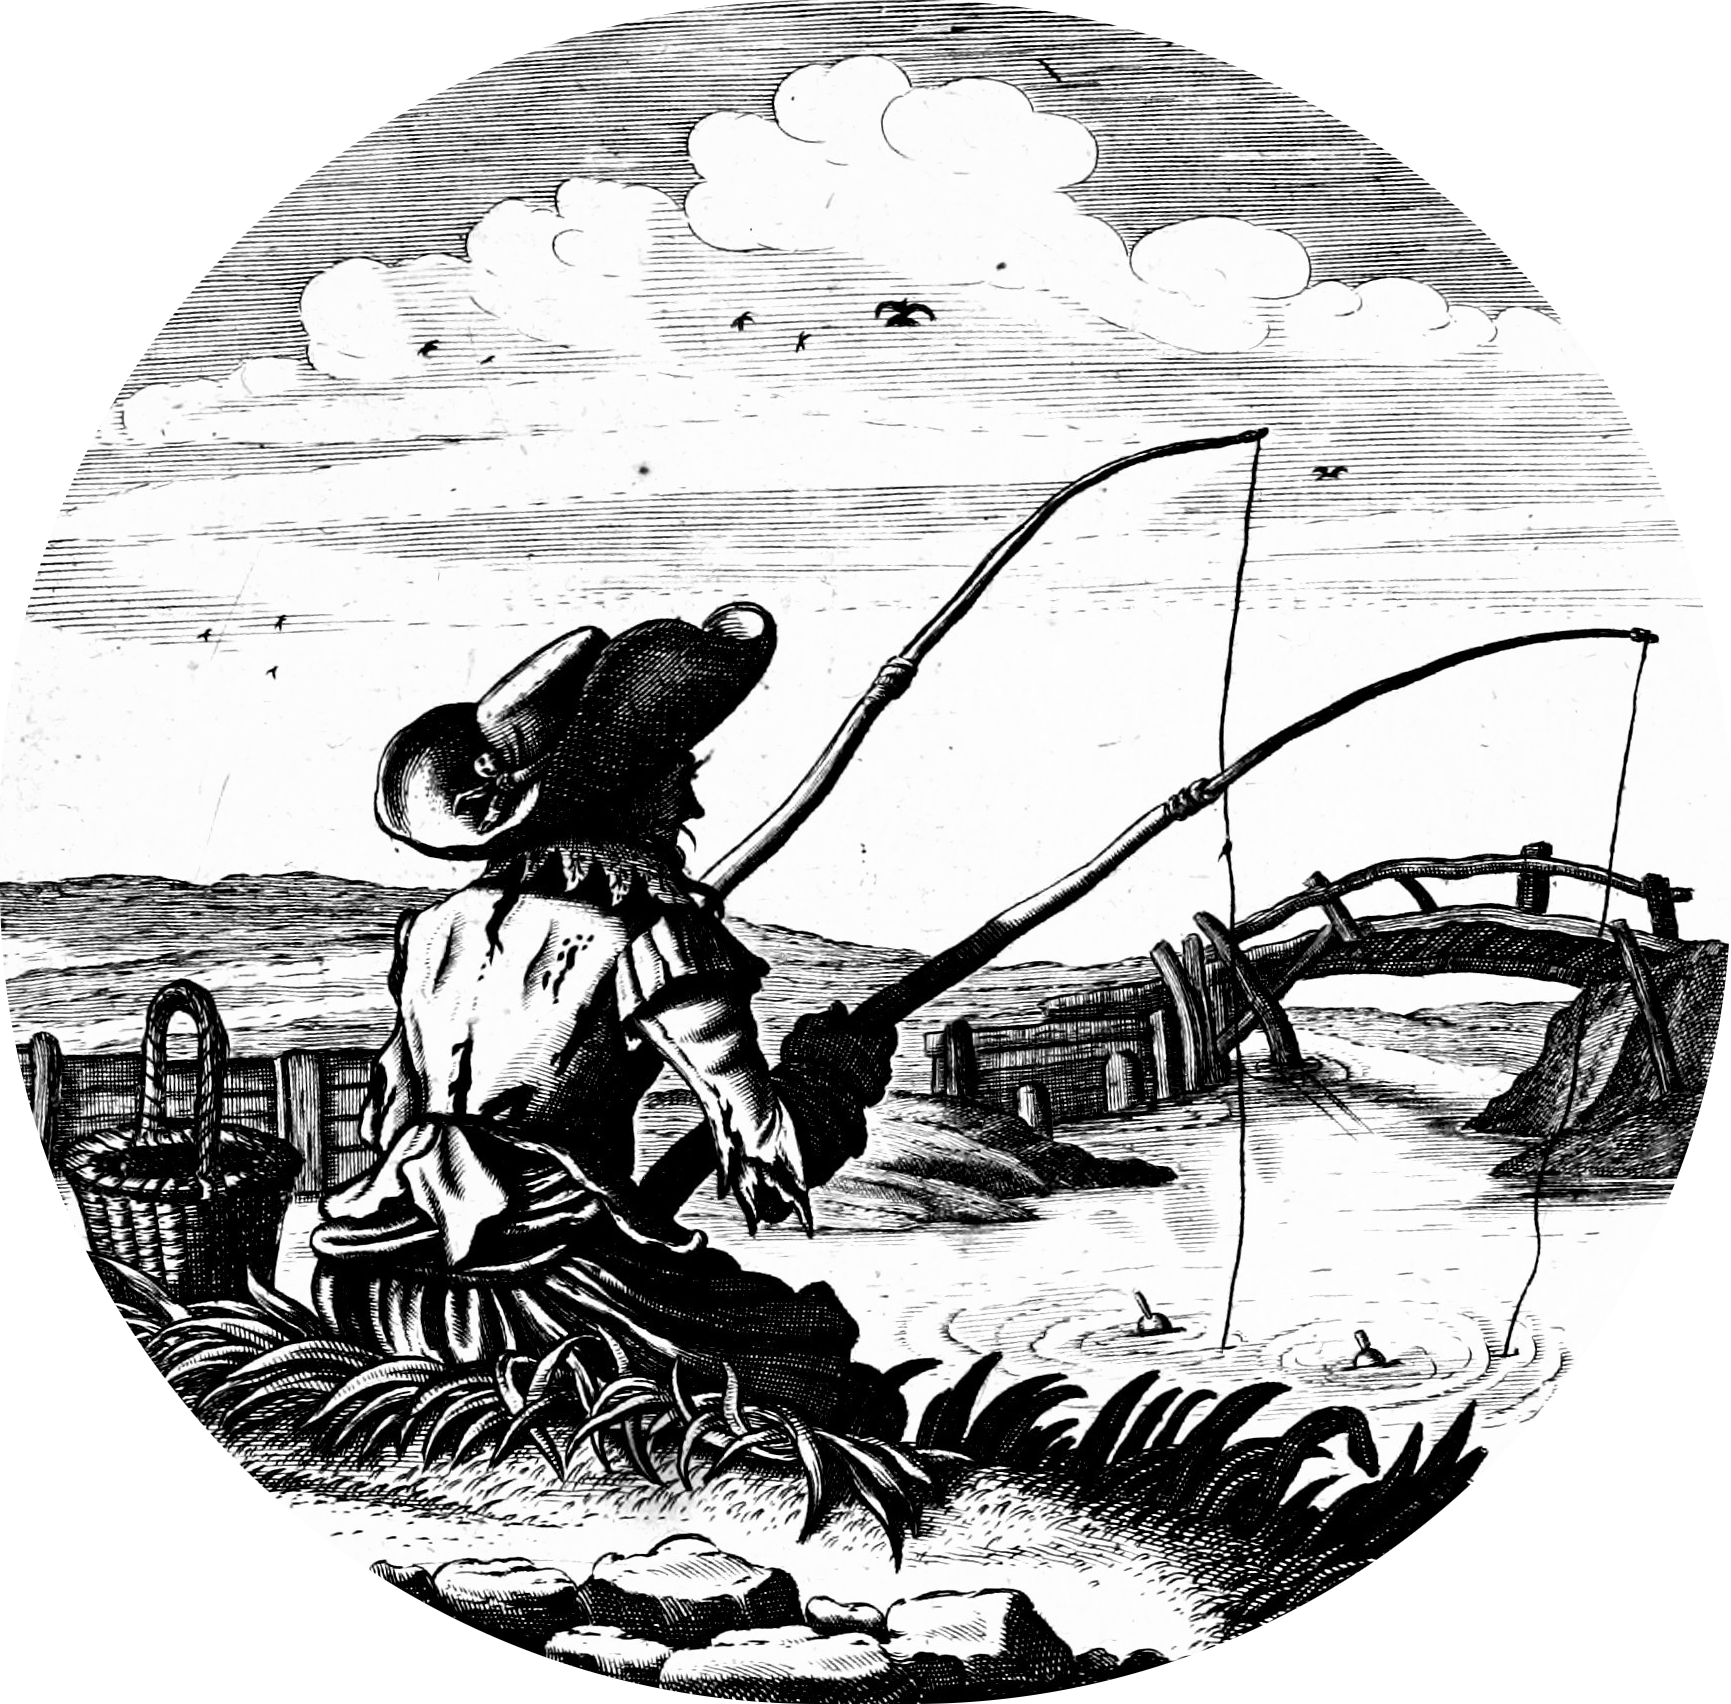
\includegraphics[width=0.9\textwidth]{images/brev41.png}
\end{center}
\breakpage